\documentclass{beamer}
\usetheme{Boadilla}
\usepackage{graphicx}
\graphicspath{ {c:/merrill/ADMB_course/Day1/images/} }

\title{Introduction to ADMB}
\subtitle{Programming for fisheries stock assessment development and application}
\author{Merrill Rudd}
\date{March 2018}
\logo{
\includegraphics[height=0.5cm]{Scaleability.png}}

\begin{document}
\begin{frame}
  \titlepage
  
\includegraphics[width=4cm,height=1.5cm]{ADMB_logo}
\end{frame}

\begin{frame}
\frametitle{Outline}
 \tableofcontents
\end{frame}

\section{Overview}
\subsection{Objectives}

\begin{frame}
\frametitle{Objectives}
Goals during this workshop
\begin{itemize}
	\item Gain fundamentals to implement and review age-structured assessments
	\item Analysis of model results in R
	\item Connecting population dynamics concepts to code
\end{itemize}
\end{frame}

\subsection{Schedule}
\begin{frame}
  \frametitle{Schedule}
  Day 1
  \begin{itemize}
  \item Introduction to ADMB, Statistical Overview
  \item Syntax, files, and output
  \item Practicing syntax, files, and output
  \item Debugging
  \end{itemize}
  Day 2
  \begin{itemize}
   \item Age-structured models
  \item Using ADMB with R
  \item Visualizing output
  \end{itemize}
  Day 3
  \begin{itemize}
  \item Using ADMB for simulation
  \item Retrospective analysis
  \item Model selection and diagnostics
  \end{itemize}
  Day 4
  \begin{itemize}
  \item Participants work with their data, work through Herring Assessment Model or other applications
    \end{itemize}
 \end{frame}

 \subsection{Course website}
 \begin{frame}
   \frametitle{Course website}
   \url{ https://github.com/merrillrudd/ADMB_course}

   Lectures and example code are available on GitHub

   Clone or download materials where you want to save them

    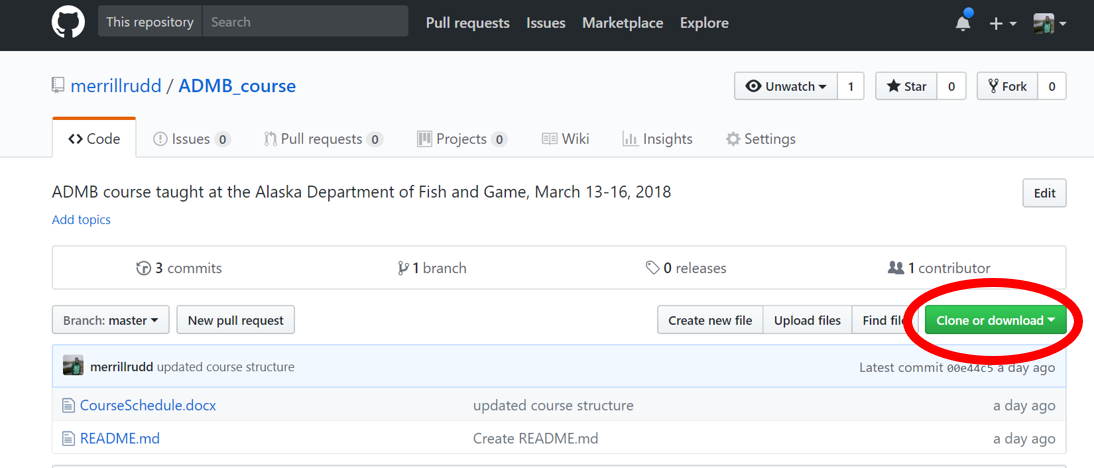
\includegraphics[width=\textwidth]{GitHub1}
 \end{frame}

 \begin{frame}
   \frametitle{Course website}
   \url{ https://github.com/merrillrudd/ADMB_course}

   ADMB installation instructions and some background material are available on the ``Wiki'' page
    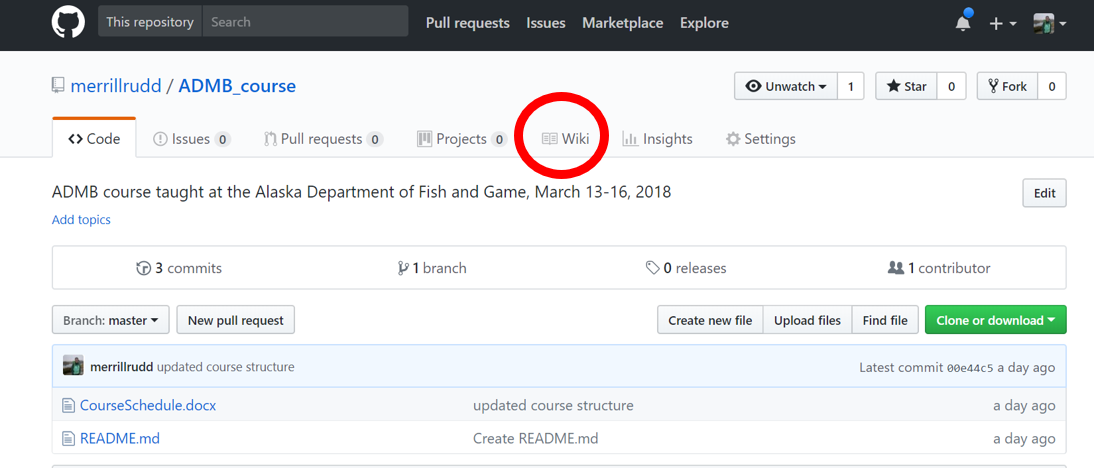
\includegraphics[width=\textwidth]{GitHub2}
  \end{frame}

  \section{ADMB Introduction}
  \begin{frame}
    \frametitle{Why use ADMB?}
    \begin{itemize}
    \item Finds the value of parameter vector that minimizes complex non-linear functions
    \item ADMB is faster, more accurate, and more stable than R optimizers (e.g. optim) with more functionality for understanding parameter uncertainty
    \end{itemize}
  \end{frame}

  \subsection{Developing a model and likelihood}
  \begin{frame}
    \frametitle{Maximum likelihood}
    \begin{itemize}
    \item Given a set of data and probability model, maximum likelihood chooses the values of parameters that make the data ``most likely''
    \item  Likelihood of the data \textit{D} given parameter(s) \textit{p} is the probability of the data given the parameter(s):
    \[ $${L(D $\mid$ p) $\approx$ Prob(D $\mid$ p)}$$  \]
   \end{itemize}
   \textbf{Probability} = knowing parameters, predicting data
   
    \textbf{Likelihood} = knowing data, estimating parameters
  \end{frame}

  % \begin{frame}
  %   \frametitle{Likelihood basics}
  %   \begin{itemize}
  %   \item If the data consists of two parts \textit{D_1} and \textit{D_2}, the likelihood of the data \[{D = D_1 + D_2}\] is the product of the likelihoods of each \textit{D_1} and \textit{D_2}:
  %   % \[  $${L(D $\mid$ p)} = {L(D_1 $\mid$ p)}{L(D_2 $\mid$ p)}$$  \]
  %  % \item \textit{D_1} and \textit{D_2} can be two data points or two data types, for example in integrated models (e.g. tag resigting, abundance index, etc.)
  %   \end{itemize}
  % \end{frame}

\end{document}
